\documentclass[12pt]{article}

\usepackage{enumitem}
\usepackage{hyperref}
\usepackage{amsthm}
\usepackage{tikz}
\usepackage{amsmath}
\usepackage{color}
\usepackage{bm}
\usepackage{array}
\usepackage{amssymb}

\newtheoremstyle{parenbold} % Name
  {2\parskip}           % Space above
  {}                    % Space below
  {}  % Body font
  {}                    % Indent amount
  {\bfseries}           % Theorem head font
  {}                    % Punctuation after theorem head
  { }                 % Space after theorem head
  {\thmnumber{#2 }\thmname{#1.\newline}\thmnote{\bfseries{#3} |}} % Theorem head spec
  
\makeatletter
\g@addto@macro\bfseries{\boldmath}
\makeatother

\theoremstyle{parenbold}
\newtheorem{definition}{Definition}[section]

\newtheorem{exmp}{Example}[section]

\newtheorem{observation}{Observation}[section]

\newtheorem{lemma}{Lemma}[section]

\newtheorem{theorem}{Theorem}[section]

\title{C\&O URA Spring 2017}
\author{Zach Dockstader}

\begin{document}
\maketitle

\tableofcontents

\section{Inertia Bounds}

\subsection{Introduction on Inertia Bounds}
\theoremstyle{definition}
\begin{definition}[Independent Set]
An independent set is a set of vertices belonging to a graph in which no two vertices are adjacent.
\end{definition}
\begin{exmp}
Consider the following graph:\\
\\
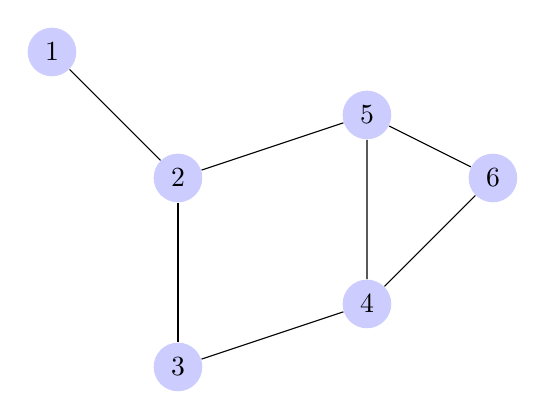
\begin{tikzpicture}
[scale=.8,every node/.style={circle,fill=blue!20}]
\node (n1) at (1,10) {1};
\node (n2) at (3,8) {2};
\node (n3) at (3,5) {3};
\node (n4) at (6,6) {4};
\node (n5) at (6,9) {5};
\node (n6) at (8,8) {6};
\foreach \from/\to in {n1/n2,n2/n3,n2/n5,n3/n4,n5/n4,n5/n6,n4/n6}
\draw (\from) -- (\to);
\end{tikzpicture}

An example of an independent set in this graph is:\\
\\
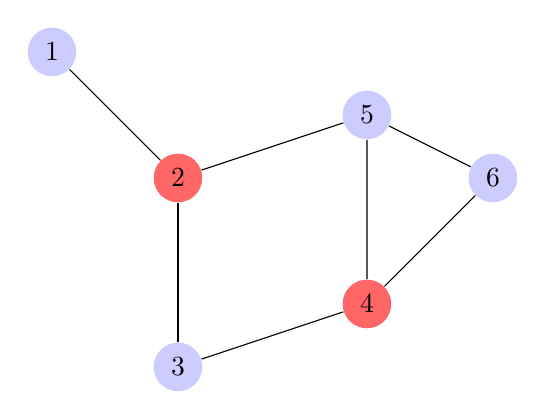
\begin{tikzpicture}
[scale=.8,every node/.style={circle,fill=blue!20}]
\node (n1) at (1,10) {1};
\node[fill=red!60] (n2) at (3,8) {2};
\node (n3) at (3,5) {3};
\node[fill=red!60] (n4) at (6,6) {4};
\node (n5) at (6,9) {5};
\node (n6) at (8,8) {6};
\foreach \from/\to in {n1/n2,n2/n3,n2/n5,n3/n4,n5/n4,n5/n6,n4/n6}
\draw (\from) -- (\to);
\end{tikzpicture}

However, often the independent set we are most interested in finding is the largest one:\\
\\
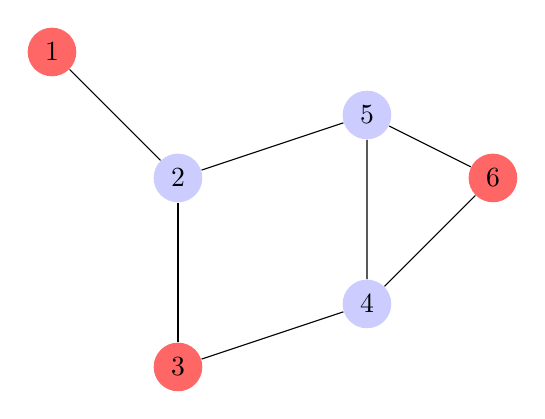
\begin{tikzpicture}
[scale=.8,every node/.style={circle,fill=blue!20}]
\node[fill=red!60] (n1) at (1,10) {1};
\node (n2) at (3,8) {2};
\node[fill=red!60] (n3) at (3,5) {3};
\node (n4) at (6,6) {4};
\node (n5) at (6,9) {5};
\node[fill=red!60] (n6) at (8,8) {6};
\foreach \from/\to in {n1/n2,n2/n3,n2/n5,n3/n4,n5/n4,n5/n6,n4/n6}
\draw (\from) -- (\to);
\end{tikzpicture}
\end{exmp}
\begin{definition}[Independence Number]
The independence number of a graph $G$, denoted $\alpha(G)$, is the size of the largest independent set of $G$.
\end{definition}

\begin{definition}[Weight Matrix]
The weight matrix of a graph $G$, is a matrix defined by:

\begin{equation}
    W_{i,j} = 
    \begin{cases}
        c_{i,j} & \mbox{if $v_i$ and $v_j$ are adjacent} \\
        0 & \mbox{otherwise}
    \end{cases}
\end{equation}
with $v_i$ a vertice of $G$ and $c_{i,j}$, a constant.

The weight matrix of a graph, is identical to an adjacency matrix, except where there was a 1 in the matrix at entry $A_{i,j}$ if vertices $v_i$ and $v_j$ were adjacent, there is now a constant indicating a weighting for the edge between $v_i$ and $v_j$.

\end{definition}

For any graph $G$, there exists a bound on $\alpha(G)$, known as the Cvetkovi\'c bound (also referred to as the Interia Bound). This bound provides a relationship between $\alpha(G)$ and the number of positive, negative, and zero eigenvalues of the weight matrix, $W$, associated with $G$. The Cvetkovi\'c bound of $G$, is:

\begin{equation}
\alpha(G) \leq \min\{|G| - n_+(W),|G|-n_-(W)\}
\end{equation}

Where $n_+(W)$ and $n_-(W)$ denote the number of positive and negative eigenvalues of $W$, respectively.

To prove this, we first need to introduce a result that comes from the Eigenvalue Interlacing Theorem:

\begin{theorem}[Corollary of Eigenvalue Interlacing Theorem]
\label{interlacing}
Let $A$ be an $n\times n$ real symmetric matrix with eigenvalues $\lambda_1 \geq \lambda_2 \geq \ldots \geq \lambda_n$ and let $C$ be a $k\times k$ principal submatrix of $A$ with eigenvalues $\tau_1 \geq \tau_2 \geq \ldots \geq \tau_k$. Then $\lambda_i \geq \tau_i$ for all $i$ $\in \{1,\ldots ,k\}$. \cite{sinkovic2016graph}
\end{theorem}

\begin{definition}[Principal Submatrix]
The principal submatrix of an $n\times n$ matrix $A$ is the submatrix obtained where if $row_i$ is excluded in the submatrix, then $column_i$ is excluded as well. Note that all principal submatrices of a weight matrix $W$, correspond to an induced subgraph in the graph represented by $W$.
\end{definition}

\begin{exmp}
The following is an example of a principal submatrix in relation to graph theory.

Consider the following graph:

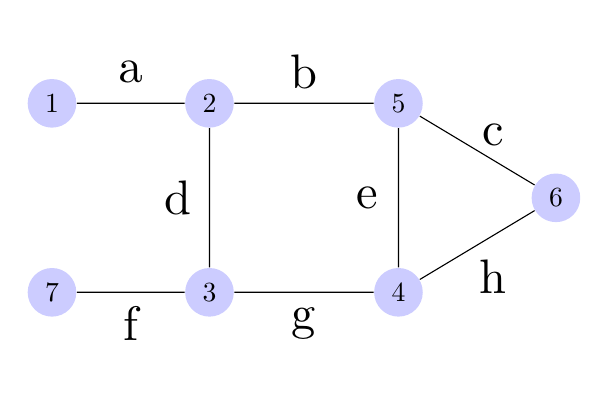
\begin{tikzpicture}
[scale=.8,every node/.style={circle,fill=blue!20}]
\node[scale=1.75,fill=white] (a) at (2.75,9.5) {a};
\node[scale=1.75,fill=white] (b) at (5.5,9.5) {b};
\node[scale=1.75,fill=white] (c) at (8.5,8.5) {c};
\node[scale=1.75,fill=white] (d) at (3.5,7.5) {d};
\node[scale=1.75,fill=white] (e) at (6.5,7.5) {e};
\node[scale=1.75,fill=white] (f) at (2.75,5.5) {f};
\node[scale=1.75,fill=white] (g) at (5.5,5.5) {g};
\node[scale=1.75,fill=white] (h) at (8.5,6.25) {h};
\node (n1) at (1.5,9) {1};
\node (n2) at (4,9) {2};
\node (n3) at (4,6) {3};
\node (n4) at (7,6) {4};
\node (n5) at (7,9) {5};
\node (n6) at (9.5,7.5) {6};
\node (n7) at (1.5,6) {7};
\foreach \from/\to in {n1/n2,n2/n3,n2/n5,n3/n4,n5/n4,n5/n6,n4/n6,n3/n7}
\draw (\from) -- (\to);
\end{tikzpicture}

and corresponding weight matrix:

$
\begin{bmatrix}
0 & a & 0 & 0 & 0 & 0 & 0 \\
a & 0 & d & 0 & b & 0 & 0 \\
0 & d & 0 & g & 0 & 0 & f \\
0 & 0 & g & 0 & e & h & 0 \\
0 & b & 0 & e & 0 & c & 0 \\
0 & 0 & 0 & h & c & 0 & 0 \\
0 & 0 & f & 0 & 0 & 0 & 0 \\
\end{bmatrix}
$
\\
\\
We can see the following principal submatrix and corresponding induced subgraph:

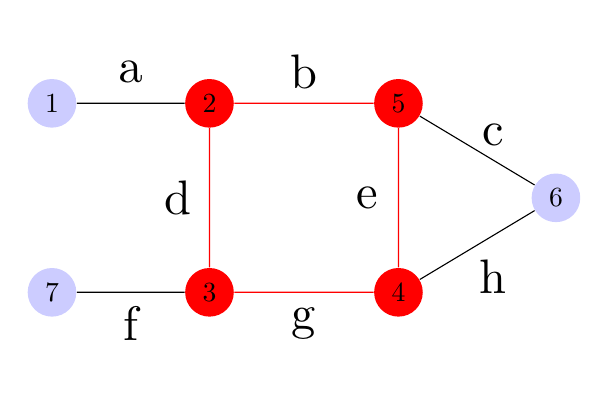
\begin{tikzpicture}
[scale=.8,every node/.style={circle,fill=blue!20}]
\node[scale=1.75,fill=white] (a) at (2.75,9.5) {a};
\node[scale=1.75,fill=white] (b) at (5.5,9.5) {b};
\node[scale=1.75,fill=white] (c) at (8.5,8.5) {c};
\node[scale=1.75,fill=white] (d) at (3.5,7.5) {d};
\node[scale=1.75,fill=white] (e) at (6.5,7.5) {e};
\node[scale=1.75,fill=white] (f) at (2.75,5.5) {f};
\node[scale=1.75,fill=white] (g) at (5.5,5.5) {g};
\node[scale=1.75,fill=white] (h) at (8.5,6.25) {h};
\node (n1) at (1.5,9) {1};
\node[fill=red] (n2) at (4,9) {2};
\node[fill=red] (n3) at (4,6) {3};
\node[fill=red] (n4) at (7,6) {4};
\node[fill=red] (n5) at (7,9) {5};
\node (n6) at (9.5,7.5) {6};
\node (n7) at (1.5,6) {7};
\foreach \from/\to in {n1/n2,n5/n6,n4/n6,n3/n7}
\draw (\from) -- (\to);
\draw[red](n2) -- (n5);
\draw[red](n2) -- (n3);
\draw[red](n3) -- (n4);
\draw[red](n4) -- (n5);
\end{tikzpicture}

$
\begin{bmatrix}
0 & a & 0 & 0 & 0 & 0 & 0 \\
a & \color{red}0 & \color{red}d & \color{red}0 & \color{red}b & 0 & 0 \\
0 & \color{red}d & \color{red}0 & \color{red}g & \color{red}0 & 0 & f \\
0 & \color{red}0 & \color{red}g & \color{red}0 & \color{red}e & h & 0 \\
0 & \color{red}b & \color{red}0 & \color{red}e & \color{red}0 & c & 0 \\
0 & 0 & 0 & h & c & 0 & 0 \\
0 & 0 & f & 0 & 0 & 0 & 0 \\
\end{bmatrix}
$
\\

As well, we see the following principal submatrix of an independent set of the graph:

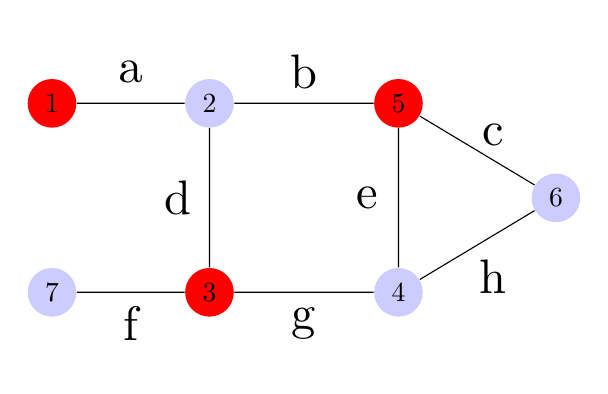
\begin{tikzpicture}
[scale=.8,every node/.style={circle,fill=blue!20}]
\node[scale=1.75,fill=white] (a) at (2.75,9.5) {a};
\node[scale=1.75,fill=white] (b) at (5.5,9.5) {b};
\node[scale=1.75,fill=white] (c) at (8.5,8.5) {c};
\node[scale=1.75,fill=white] (d) at (3.5,7.5) {d};
\node[scale=1.75,fill=white] (e) at (6.5,7.5) {e};
\node[scale=1.75,fill=white] (f) at (2.75,5.5) {f};
\node[scale=1.75,fill=white] (g) at (5.5,5.5) {g};
\node[scale=1.75,fill=white] (h) at (8.5,6.25) {h};
\node[fill=red] (n1) at (1.5,9) {1};
\node (n2) at (4,9) {2};
\node[fill=red] (n3) at (4,6) {3};
\node (n4) at (7,6) {4};
\node[fill=red] (n5) at (7,9) {5};
\node (n6) at (9.5,7.5) {6};
\node (n7) at (1.5,6) {7};
\foreach \from/\to in {n1/n2,n2/n3,n2/n5,n3/n4,n5/n4,n5/n6,n4/n6,n3/n7}
\draw (\from) -- (\to);
\end{tikzpicture}

$
\begin{bmatrix}
\color{red}0 & a & \color{red}0 & 0 & \color{red}0 & 0 & 0 \\
a & 0 & d & 0 & b & 0 & 0 \\
\color{red}0 & d & \color{red}0 & g & \color{red}0 & 0 & f \\
0 & 0 & g & 0 & e & h & 0 \\
\color{red}0 & b & \color{red}0 & e & \color{red}0 & c & 0 \\
0 & 0 & 0 & h & c & 0 & 0 \\
0 & 0 & f & 0 & 0 & 0 & 0 \\
\end{bmatrix}
$
\\
\end{exmp}

Now to prove the Cvetkovi\'c Bound:

\begin{theorem}[Cvetkovi\'c Bound]
Let $G$ be a graph on n vertices, and $W$ be the weight matrix of $G$. Then the following inequality holds:
\begin{equation}
\alpha(G) \leq \min\{|G| - n_+(W),|G|-n_-(W)\}
\end{equation}
\end{theorem}

\begin{proof}\footnote{Interesting Graphs and their Colourings, unpublished lecture notes C. Godsil (2004)}
Let $H$ be the subgraph of $G$ formed by the vertices in an independent set of size s. Then $H$ is an induced subgraph of $G$ and all eigenvalues of the principal submatrix $W(H)$ are 0 since the principal submatrix will just be a zero matrix. Let $\lambda_i$ denote the $i$th largest eigenvalue of $W$ and $\tau_i$ denote the $i$th larest eigenvalue of $W(H)$. Now, by interlacing, we have,
\begin{equation}
\lambda_i \geq \tau_i = 0 \text{ for all i } \in \{1,\ldots ,s\}
\end{equation}

and so 
\begin{equation}
n - n_-(W) = n_+(W) + n_0(W) \geq s
\end{equation}
Also, note that by negating $W$, the positive eigenvalues become negative eigenvalues and vice versa. Thus,
\begin{equation}
n - n_+(W) = n - n_-(-W),
\end{equation}
However, the principal submatrix corresponding to $H$ in $-W$ is still the zero matrix and thus has all zero eigenvalues. Thus, by interlacing, we get a similar result as above, 
\begin{equation}
n - n_+(W) = n - n_-(-W) = n_+(-W) + n_0(-W) \geq s
\end{equation}

Therefore, both $n - n_+(W)$ and $n - n_-(W)$ are greater than or equal to s. Since s is the size of the idependent set, we can see that letting s = $\alpha(G)$, we get:

\begin{equation}
\alpha(G) \leq \min\{|G| - n_+(W),|G|-n_-(W)\}
\end{equation}

\end{proof}

\subsection{Graphs with Tight Inertia Bounds}

\subsubsection{Perfect Graphs}

\begin{definition}[Chromatic Number]
The chromatic number of a graph, $\chi(G)$, is the minimum number of colours needed in a proper colouring of G. \cite{elzinga2007minimum}
\end{definition}

\begin{exmp}
Consider the following graph:
\\

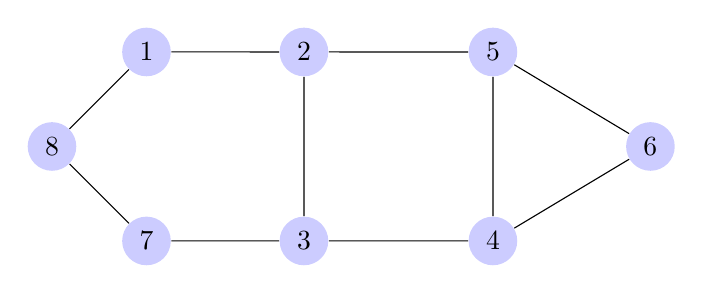
\begin{tikzpicture}
[scale=.8,every node/.style={circle,fill=blue!20}]
\node (n1) at (1.5,9) {1};
\node (n2) at (4,9) {2};
\node (n3) at (4,6) {3};
\node (n4) at (7,6) {4};
\node (n5) at (7,9) {5};
\node (n6) at (9.5,7.5) {6};
\node (n7) at (1.5,6) {7};
\node (n8) at (0,7.5) {8};
\foreach \from/\to in {n1/n2,n2/n3,n2/n5,n3/n4,n5/n4,n5/n6,n4/n6,n3/n7,n7/n8,n1/n8}
\draw (\from) -- (\to);
\end{tikzpicture}

An example of a colouring would be:
\\

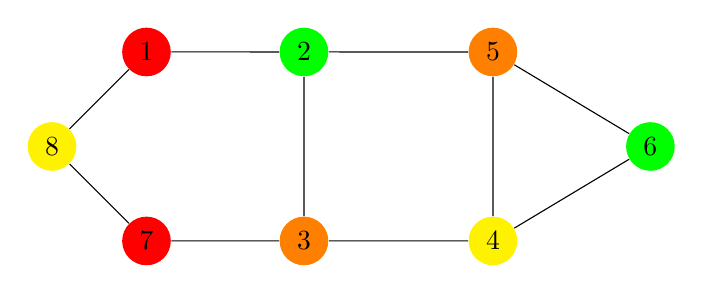
\begin{tikzpicture}
[scale=.8,every node/.style={circle,fill=blue!20}]
\node[fill=red] (n1) at (1.5,9) {1};
\node[fill=green] (n2) at (4,9) {2};
\node[fill=orange] (n3) at (4,6) {3};
\node[fill=yellow] (n4) at (7,6) {4};
\node[fill=orange] (n5) at (7,9) {5};
\node[fill=green] (n6) at (9.5,7.5) {6};
\node[fill=red] (n7) at (1.5,6) {7};
\node[fill=yellow] (n8) at (0,7.5) {8};
\foreach \from/\to in {n1/n2,n2/n3,n2/n5,n3/n4,n5/n4,n5/n6,n4/n6,n3/n7,n7/n8,n1/n8}
\draw (\from) -- (\to);
\end{tikzpicture}

However, $\chi(G)$ for this graph is 3:
\\

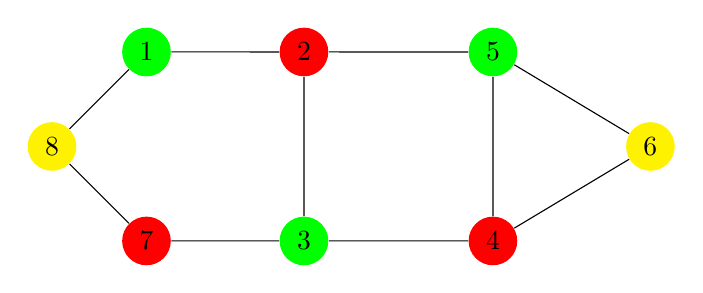
\begin{tikzpicture}
[scale=.8,every node/.style={circle,fill=blue!20}]
\node[fill=green] (n1) at (1.5,9) {1};
\node[fill=red] (n2) at (4,9) {2};
\node[fill=green] (n3) at (4,6) {3};
\node[fill=red] (n4) at (7,6) {4};
\node[fill=green] (n5) at (7,9) {5};
\node[fill=yellow] (n6) at (9.5,7.5) {6};
\node[fill=red] (n7) at (1.5,6) {7};
\node[fill=yellow] (n8) at (0,7.5) {8};
\foreach \from/\to in {n1/n2,n2/n3,n2/n5,n3/n4,n5/n4,n5/n6,n4/n6,n3/n7,n7/n8,n1/n8}
\draw (\from) -- (\to);
\end{tikzpicture}

\end{exmp}

\begin{definition}[Clique]
An m-clique in a graph is a complete subgraph on m vertices. \cite{elzinga2007minimum}

The clique number, $\omega(G)$, is the number of vertices in a maximum clique of $G$.

\end{definition}

\begin{definition}[Clique Cover]
A Clique Cover of the vertex set $V(G)$ of a graph $G$ is a set of cliques $C$, such that each vertex is in at least one clique in $C$. 

The clique cover number, $\theta(G)$ is the minimum number of cliques needed in a clique cover of $G$. \cite{elzinga2007minimum}

\end{definition}

\begin{exmp}
Consider the following graph:
\\
\\
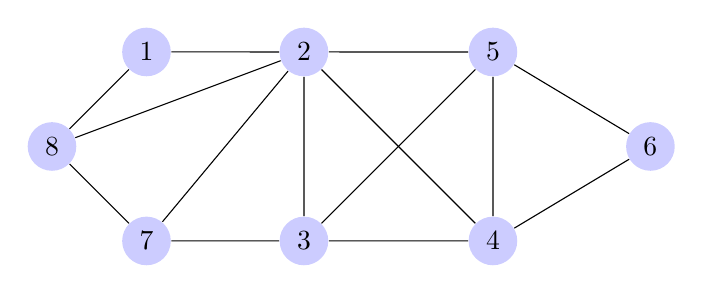
\begin{tikzpicture}
[scale=.8,every node/.style={circle,fill=blue!20}]
\node (n1) at (1.5,9) {1};
\node (n2) at (4,9) {2};
\node (n3) at (4,6) {3};
\node (n4) at (7,6) {4};
\node (n5) at (7,9) {5};
\node (n6) at (9.5,7.5) {6};
\node (n7) at (1.5,6) {7};
\node (n8) at (0,7.5) {8};
\foreach \from/\to in {n1/n2,n2/n3,n2/n5,n3/n4,n5/n4,n5/n6,n4/n6,n3/n7,n7/n8,n1/n8,n2/n4,n3/n5,n2/n7,n2/n8}
\draw (\from) -- (\to);
\end{tikzpicture}

A possible clique covering is:
\\
\\
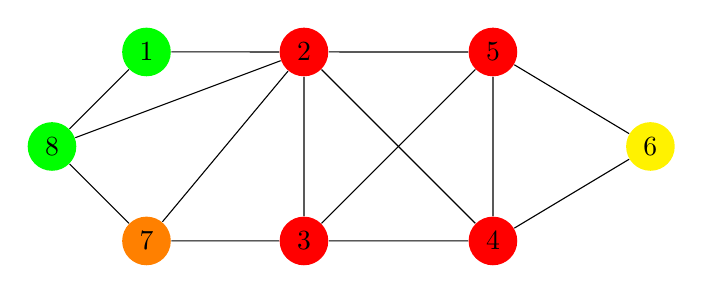
\begin{tikzpicture}
[scale=.8,every node/.style={circle,fill=blue!20}]
\node[fill=green] (n1) at (1.5,9) {1};
\node[fill=red] (n2) at (4,9) {2};
\node[fill=red] (n3) at (4,6) {3};
\node[fill=red] (n4) at (7,6) {4};
\node[fill=red] (n5) at (7,9) {5};
\node[fill=yellow] (n6) at (9.5,7.5) {6};
\node[fill=orange] (n7) at (1.5,6) {7};
\node[fill=green] (n8) at (0,7.5) {8};
\foreach \from/\to in {n1/n2,n2/n3,n2/n5,n3/n4,n5/n4,n5/n6,n4/n6,n3/n7,n7/n8,n1/n8,n2/n4,n3/n5,n2/n7,n2/n8}
\draw (\from) -- (\to);
\end{tikzpicture}

However, we can find that $\theta(G)$ is equal to 3 (smallest I could find):
\\
\\
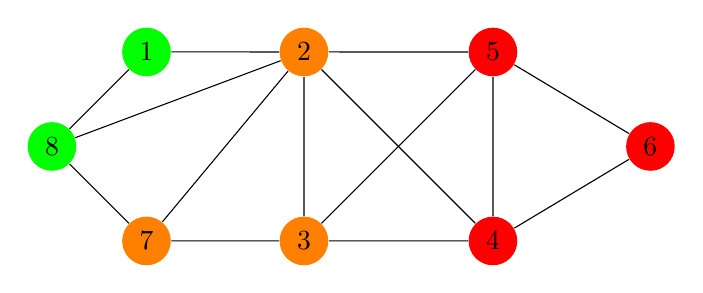
\begin{tikzpicture}
[scale=.8,every node/.style={circle,fill=blue!20}]
\node[fill=green] (n1) at (1.5,9) {1};
\node[fill=orange] (n2) at (4,9) {2};
\node[fill=orange] (n3) at (4,6) {3};
\node[fill=red] (n4) at (7,6) {4};
\node[fill=red] (n5) at (7,9) {5};
\node[fill=red] (n6) at (9.5,7.5) {6};
\node[fill=orange] (n7) at (1.5,6) {7};
\node[fill=green] (n8) at (0,7.5) {8};
\foreach \from/\to in {n1/n2,n2/n3,n2/n5,n3/n4,n5/n4,n5/n6,n4/n6,n3/n7,n7/n8,n1/n8,n2/n4,n3/n5,n2/n7,n2/n8}
\draw (\from) -- (\to);
\end{tikzpicture}

As well, the clique number, $\omega(G)$, is 4:
\\
\\
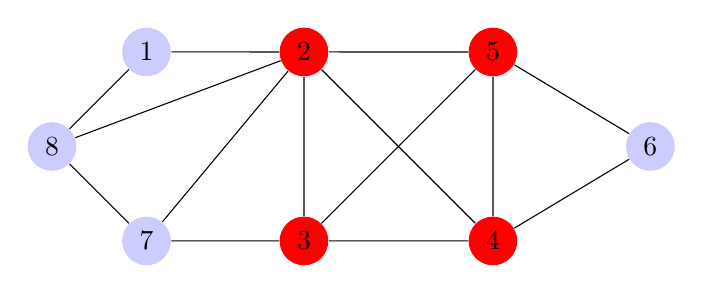
\begin{tikzpicture}
[scale=.8,every node/.style={circle,fill=blue!20}]
\node (n1) at (1.5,9) {1};
\node[fill=red] (n2) at (4,9) {2};
\node[fill=red] (n3) at (4,6) {3};
\node[fill=red] (n4) at (7,6) {4};
\node[fill=red] (n5) at (7,9) {5};
\node (n6) at (9.5,7.5) {6};
\node (n7) at (1.5,6) {7};
\node (n8) at (0,7.5) {8};
\foreach \from/\to in {n1/n2,n2/n3,n2/n5,n3/n4,n5/n4,n5/n6,n4/n6,n3/n7,n7/n8,n1/n8,n2/n4,n3/n5,n2/n7,n2/n8}
\draw (\from) -- (\to);
\end{tikzpicture}

\end{exmp}

\begin{definition}[Perfect Graph]
A graph G is perfect if $\chi(G) = \omega(G)$ for all induced subgraphs, H, of G.

\end{definition}

\begin{theorem}[Perfect Graph Theorem] \label{PGthm}
A Graph $G$ is perfect if and only if its compliment, $\overline{G}$, is also perfect.
\end{theorem}

\begin{observation} \label{obs1}
For a graph $G$, $\omega(G) = \alpha(\overline{G})$
\end{observation}

\begin{exmp}
Consider the following graph, $G$:

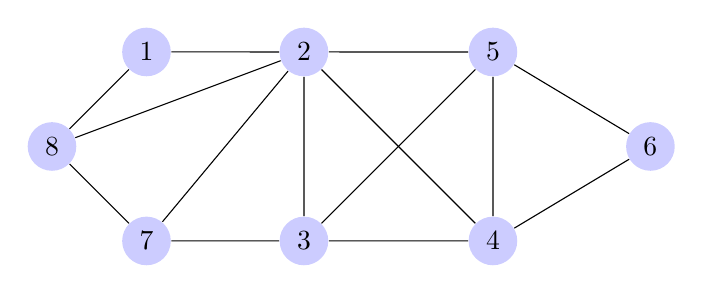
\begin{tikzpicture}
[scale=.8,every node/.style={circle,fill=blue!20}]
\node (n1) at (1.5,9) {1};
\node (n2) at (4,9) {2};
\node (n3) at (4,6) {3};
\node (n4) at (7,6) {4};
\node (n5) at (7,9) {5};
\node (n6) at (9.5,7.5) {6};
\node (n7) at (1.5,6) {7};
\node (n8) at (0,7.5) {8};
\foreach \from/\to in {n1/n2,n2/n3,n2/n5,n3/n4,n5/n4,n5/n6,n4/n6,n3/n7,n7/n8,n1/n8,n2/n4,n3/n5,n2/n7,n2/n8}
\draw (\from) -- (\to);
\end{tikzpicture}

We see that the largest clique in $G$ is:

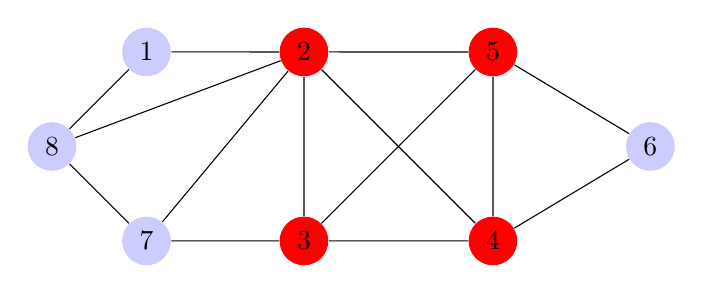
\begin{tikzpicture}
[scale=.8,every node/.style={circle,fill=blue!20}]
\node (n1) at (1.5,9) {1};
\node[fill=red] (n2) at (4,9) {2};
\node[fill=red] (n3) at (4,6) {3};
\node[fill=red] (n4) at (7,6) {4};
\node[fill=red] (n5) at (7,9) {5};
\node (n6) at (9.5,7.5) {6};
\node (n7) at (1.5,6) {7};
\node (n8) at (0,7.5) {8};
\foreach \from/\to in {n1/n2,n2/n3,n2/n5,n3/n4,n5/n4,n5/n6,n4/n6,n3/n7,n7/n8,n1/n8,n2/n4,n3/n5,n2/n7,n2/n8}
\draw (\from) -- (\to);
\end{tikzpicture}

Thus, $W(G)$ is 4.

Now consider $G$'s compliment, $\overline{G}$:

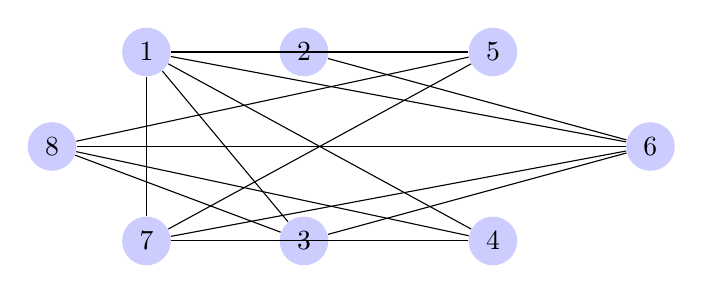
\begin{tikzpicture}
[scale=.8,every node/.style={circle,fill=blue!20}]
\node (n1) at (1.5,9) {1};
\node (n2) at (4,9) {2};
\node (n3) at (4,6) {3};
\node (n4) at (7,6) {4};
\node (n5) at (7,9) {5};
\node (n6) at (9.5,7.5) {6};
\node (n7) at (1.5,6) {7};
\node (n8) at (0,7.5) {8};
\foreach \from/\to in {n1/n7,n1/n3,n1/n4,n1/n5,n1/n6,n2/n6,n3/n8,n3/n6,n4/n7,n4/n8,n5/n7,n5/n8,n6/n7,n6/n8}
\draw (\from) -- (\to);
\end{tikzpicture}

In $\overline{G}$, the largest independent set is:

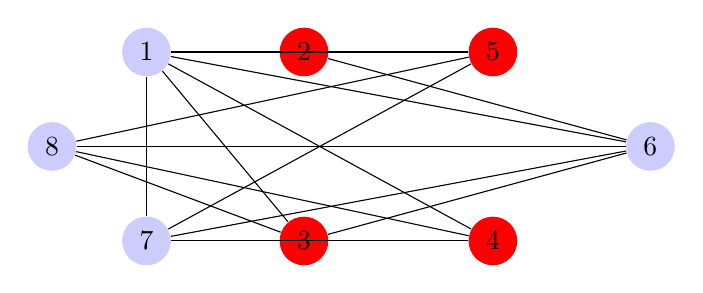
\begin{tikzpicture}
[scale=.8,every node/.style={circle,fill=blue!20}]
\node (n1) at (1.5,9) {1};
\node[fill=red] (n2) at (4,9) {2};
\node[fill=red] (n3) at (4,6) {3};
\node[fill=red] (n4) at (7,6) {4};
\node[fill=red] (n5) at (7,9) {5};
\node (n6) at (9.5,7.5) {6};
\node (n7) at (1.5,6) {7};
\node (n8) at (0,7.5) {8};
\foreach \from/\to in {n1/n7,n1/n3,n1/n4,n1/n5,n1/n6,n2/n6,n3/n8,n3/n6,n4/n7,n4/n8,n5/n7,n5/n8,n6/n7,n6/n8}
\draw (\from) -- (\to);
\end{tikzpicture}

Therefore, we see $\omega(G) = 4 = \alpha(\overline{G})$

\end{exmp}

\begin{observation} \label{obs2}
Similar to the last observation, for a graph $G$, $\theta(G) = \chi(\overline{G})$
\end{observation}

\begin{exmp}
Consider the same graph from the last example. Recall that we calculated $\theta(G)$ to be 3. Now, we can find $\chi(\overline{G})$ to be 3 as well:

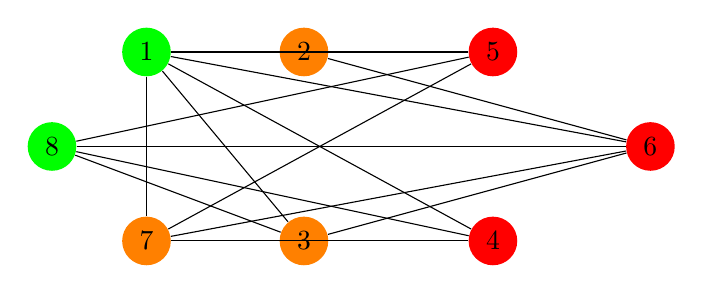
\begin{tikzpicture}
[scale=.8,every node/.style={circle,fill=blue!20}]
\node[fill=green] (n1) at (1.5,9) {1};
\node[fill=orange] (n2) at (4,9) {2};
\node[fill=orange] (n3) at (4,6) {3};
\node[fill=red] (n4) at (7,6) {4};
\node[fill=red] (n5) at (7,9) {5};
\node[fill=red] (n6) at (9.5,7.5) {6};
\node[fill=orange] (n7) at (1.5,6) {7};
\node[fill=green] (n8) at (0,7.5) {8};
\foreach \from/\to in {n1/n7,n1/n3,n1/n4,n1/n5,n1/n6,n2/n6,n3/n8,n3/n6,n4/n7,n4/n8,n5/n7,n5/n8,n6/n7,n6/n8}
\draw (\from) -- (\to);
\end{tikzpicture}

Thus, $\theta(G) = 3 = \chi(\overline{G})$

\end{exmp}

\begin{lemma} \label{lem:alphatheta}
Let $G$ be a graph. Then $\alpha(G) \leq \min\{|G| - n_+(W),|G|-n_-(W)\} \leq \theta(G)$. Thus, if $\alpha(G) = \theta(G)$, G has a tight inertia bound. 
\cite{elzinga2007minimum}
\end{lemma}

\begin{proof}
Consider a clique partition, $\mathcal{C}$, of a graph $G$. Let $\hat{A}$, denote the adjacency matrix of G where the only connected components are the cliques in $\mathcal{C}$.

Now if we consider the adjacency matrix of the complete graph, $K_n$, we see that it is equal to $J_n - I_n$ where $J_n$ is the all ones matrix. 
\end{proof}

\begin{theorem}
Every Perfect Graph, $G$, has a tight inertia bound
\end{theorem}

\begin{proof}
By the Perfect Graph Theorem (theorem \ref{PGthm}), we know that $\overline{G}$, is also perfect. Thus $\overline{G}$ satisies that $\chi(H) = \omega(H)$ for all subgraphs, $H$, of $\overline{G}$, by definition.
Thus, since $\chi(\overline{G}) = \omega(\overline{G})$, we can get from the observation \ref{obs1} and \ref{obs2}, that
\begin{equation}
\alpha(G) = \omega(\overline{G}) = \chi(\overline{G}) = \theta(G)
\end{equation}

Therefore, from lemma \ref{lem:alphatheta}, G has a tight inertia bound.
\end{proof}

\begin{theorem}[Strong Perfect Graph Theorem \cite{elzinga2007minimum}] \label{SPGT}
A graph $G$ is a perfect graph if and only if both $G$ and its complement, $\overline{G}$, do not contain a induced odd cycle of length at least 5.
\end{theorem}

\begin{observation}
Due to each perfect graph having a tight inertia bound, and the Strong Perfect Graph Theorem (theorem \ref{SPGT}), every graph not containing an induced odd cycle of length 5 or greater has a tight inertia bound.
\end{observation}

\subsubsection{Latin Square Graphs}

\subsubsection{Graphs with an Eigensharp decomposition by Stars}

\subsubsection{Summary}
In summary, the following list of graphs attain a tight inertia bound:
\begin{itemize}
	\item Graphs on 10 or fewer vertices (pg 81 \cite{elzinga2007minimum})
	\item Vertex Transitive graphs on 12 or fewer vertices (pg 81 \cite{elzinga2007minimum})
	\item Perfect Graphs
	\item Latin Square Graphs
	\item Graphs with an Eigensharp decomposition by stars
\end{itemize}

\subsection{Other Bounds on Independence Number}

\section{Algorithm to Find Graphs Lacking a Tight Inertia Bound}

\subsection{Outline of Method}

\begin{definition}[Optimal Weight Matrix]
A weight matrix, $W$, of a graph, $G$, is optimal if
\begin{equation}
\alpha(G) = \min\{|G| - n_+(W),|G| - n_-(W)\}
\end{equation}
\end{definition}

\begin{exmp}
Consider the following graph, $G$, with corresponding weight matrix $W$:

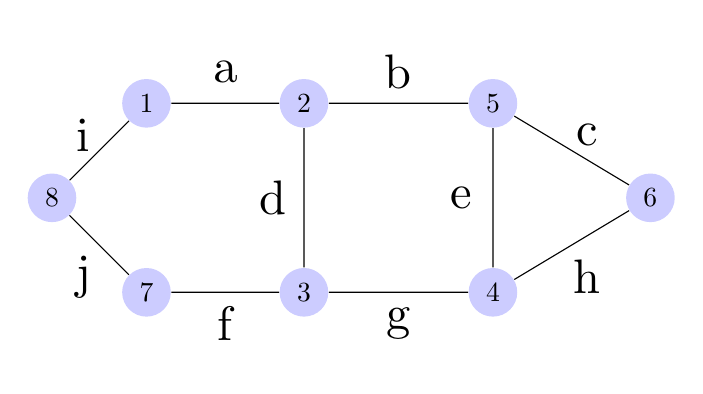
\begin{tikzpicture}
[scale=.8,every node/.style={circle,fill=blue!20}]
\node[scale=1.75,fill=white] (a) at (2.75,9.5) {a};
\node[scale=1.75,fill=white] (b) at (5.5,9.5) {b};
\node[scale=1.75,fill=white] (c) at (8.5,8.5) {c};
\node[scale=1.75,fill=white] (d) at (3.5,7.5) {d};
\node[scale=1.75,fill=white] (e) at (6.5,7.5) {e};
\node[scale=1.75,fill=white] (f) at (2.75,5.5) {f};
\node[scale=1.75,fill=white] (g) at (5.5,5.5) {g};
\node[scale=1.75,fill=white] (h) at (8.5,6.25) {h};
\node[scale=1.75,fill=white] (i) at (0.5,8.5) {i};
\node[scale=1.75,fill=white] (j) at (0.5,6.25) {j};
\node (n1) at (1.5,9) {1};
\node (n2) at (4,9) {2};
\node (n3) at (4,6) {3};
\node (n4) at (7,6) {4};
\node (n5) at (7,9) {5};
\node (n6) at (9.5,7.5) {6};
\node (n7) at (1.5,6) {7};
\node (n8) at (0,7.5) {8};
\foreach \from/\to in {n1/n2,n2/n3,n2/n5,n3/n4,n5/n4,n5/n6,n4/n6,n3/n7,n7/n8,n1/n8}
\draw (\from) -- (\to);
\end{tikzpicture}

$
\begin{bmatrix}
0 & a & 0 & 0 & 0 & 0 & 0 & i \\
a & 0 & d & 0 & b & 0 & 0 & 0\\
0 & d & 0 & g & 0 & 0 & f & 0 \\
0 & 0 & g & 0 & e & h & 0 & 0 \\
0 & b & 0 & e & 0 & c & 0 & 0 \\
0 & 0 & 0 & h & c & 0 & 0 & 0 \\
0 & 0 & f & 0 & 0 & 0 & 0 & j\\
i & 0 & 0 & 0 & 0 & 0 & j & 0\\
\end{bmatrix}
$
\\

We can see the independent number of $G$ is 3:

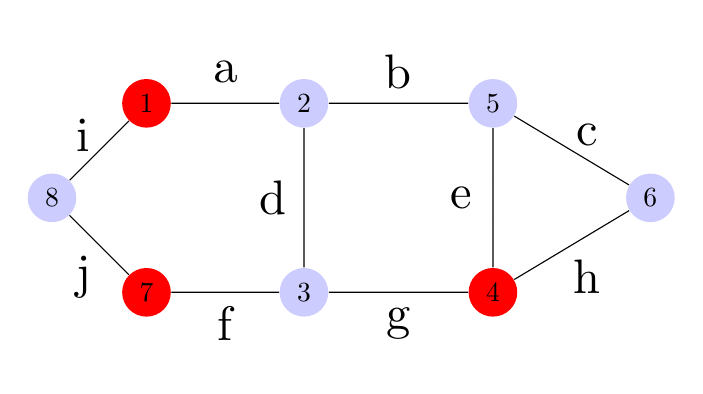
\begin{tikzpicture}
[scale=.8,every node/.style={circle,fill=blue!20}]
\node[scale=1.75,fill=white] (a) at (2.75,9.5) {a};
\node[scale=1.75,fill=white] (b) at (5.5,9.5) {b};
\node[scale=1.75,fill=white] (c) at (8.5,8.5) {c};
\node[scale=1.75,fill=white] (d) at (3.5,7.5) {d};
\node[scale=1.75,fill=white] (e) at (6.5,7.5) {e};
\node[scale=1.75,fill=white] (f) at (2.75,5.5) {f};
\node[scale=1.75,fill=white] (g) at (5.5,5.5) {g};
\node[scale=1.75,fill=white] (h) at (8.5,6.25) {h};
\node[scale=1.75,fill=white] (i) at (0.5,8.5) {i};
\node[scale=1.75,fill=white] (j) at (0.5,6.25) {j};
\node[fill=red] (n1) at (1.5,9) {1};
\node (n2) at (4,9) {2};
\node (n3) at (4,6) {3};
\node[fill=red] (n4) at (7,6) {4};
\node (n5) at (7,9) {5};
\node (n6) at (9.5,7.5) {6};
\node[fill=red] (n7) at (1.5,6) {7};
\node (n8) at (0,7.5) {8};
\foreach \from/\to in {n1/n2,n2/n3,n2/n5,n3/n4,n5/n4,n5/n6,n4/n6,n3/n7,n7/n8,n1/n8}
\draw (\from) -- (\to);
\end{tikzpicture}

Now, let G have the following weighting:

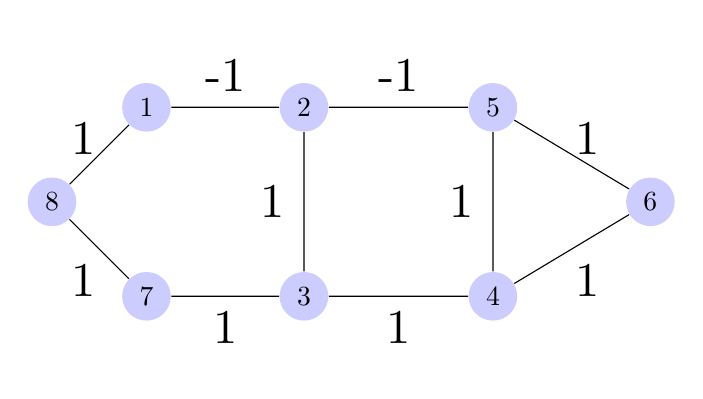
\begin{tikzpicture}
[scale=.8,every node/.style={circle,fill=blue!20}]
\node[scale=1.75,fill=white] (a) at (2.75,9.5) {-1};
\node[scale=1.75,fill=white] (b) at (5.5,9.5) {-1};
\node[scale=1.75,fill=white] (c) at (8.5,8.5) {1};
\node[scale=1.75,fill=white] (d) at (3.5,7.5) {1};
\node[scale=1.75,fill=white] (e) at (6.5,7.5) {1};
\node[scale=1.75,fill=white] (f) at (2.75,5.5) {1};
\node[scale=1.75,fill=white] (g) at (5.5,5.5) {1};
\node[scale=1.75,fill=white] (h) at (8.5,6.25) {1};
\node[scale=1.75,fill=white] (i) at (0.5,8.5) {1};
\node[scale=1.75,fill=white] (j) at (0.5,6.25) {1};
\node (n1) at (1.5,9) {1};
\node (n2) at (4,9) {2};
\node (n3) at (4,6) {3};
\node (n4) at (7,6) {4};
\node (n5) at (7,9) {5};
\node (n6) at (9.5,7.5) {6};
\node (n7) at (1.5,6) {7};
\node (n8) at (0,7.5) {8};
\foreach \from/\to in {n1/n2,n2/n3,n2/n5,n3/n4,n5/n4,n5/n6,n4/n6,n3/n7,n7/n8,n1/n8}
\draw (\from) -- (\to);
\end{tikzpicture}

$
\begin{bmatrix}
0 & -1 & 0 & 0 & 0 & 0 & 0 & 1 \\
-1 & 0 & 1 & 0 & -1 & 0 & 0 & 0\\
0 & 1 & 0 & 1 & 0 & 0 & 1 & 0 \\
0 & 0 & 1 & 0 & 1 & 1 & 0 & 0 \\
0 & -1 & 0 & 1 & 0 & 1 & 0 & 0 \\
0 & 0 & 0 & 1 & 1 & 0 & 0 & 0 \\
0 & 0 & 1 & 0 & 0 & 0 & 0 & 1\\
1 & 0 & 0 & 0 & 0 & 0 & 1 & 0\\
\end{bmatrix}
$
\\

Finding the eigenvalues of $W$, we find there are 3 positive eigenvalues and 5 negative eigenvalues. Thus, we see for this weight matrix we have:

\begin{equation}
\begin{split}
\alpha(G) & = \min\{|G| - n_+(W),|G| - n_-(W)\} \\
& = \min\{8 - 3,8 - 5\} \\
& = \min\{5,3\} \\
& = 3
\end{split}
\end{equation}

Therefore, this is an optimal weight matrix of G.

Now consider the following weighting for the same graph:

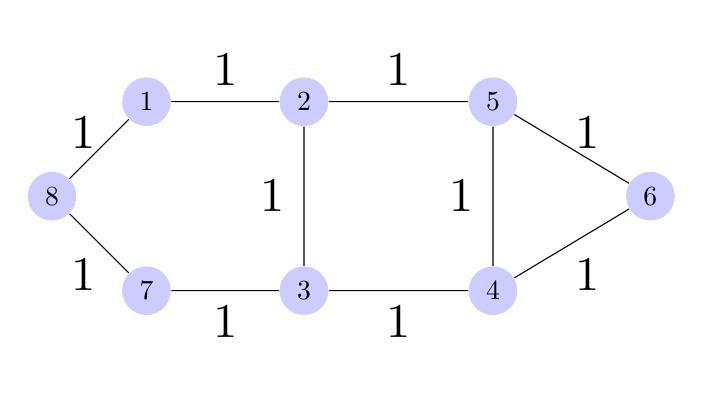
\begin{tikzpicture}
[scale=.8,every node/.style={circle,fill=blue!20}]
\node[scale=1.75,fill=white] (a) at (2.75,9.5) {1};
\node[scale=1.75,fill=white] (b) at (5.5,9.5) {1};
\node[scale=1.75,fill=white] (c) at (8.5,8.5) {1};
\node[scale=1.75,fill=white] (d) at (3.5,7.5) {1};
\node[scale=1.75,fill=white] (e) at (6.5,7.5) {1};
\node[scale=1.75,fill=white] (f) at (2.75,5.5) {1};
\node[scale=1.75,fill=white] (g) at (5.5,5.5) {1};
\node[scale=1.75,fill=white] (h) at (8.5,6.25) {1};
\node[scale=1.75,fill=white] (i) at (0.5,8.5) {1};
\node[scale=1.75,fill=white] (j) at (0.5,6.25) {1};
\node (n1) at (1.5,9) {1};
\node (n2) at (4,9) {2};
\node (n3) at (4,6) {3};
\node (n4) at (7,6) {4};
\node (n5) at (7,9) {5};
\node (n6) at (9.5,7.5) {6};
\node (n7) at (1.5,6) {7};
\node (n8) at (0,7.5) {8};
\foreach \from/\to in {n1/n2,n2/n3,n2/n5,n3/n4,n5/n4,n5/n6,n4/n6,n3/n7,n7/n8,n1/n8}
\draw (\from) -- (\to);
\end{tikzpicture}

$
\begin{bmatrix}
0 & 1 & 0 & 0 & 0 & 0 & 0 & 1 \\
1 & 0 & 1 & 0 & 1 & 0 & 0 & 0\\
0 & 1 & 0 & 1 & 0 & 0 & 1 & 0 \\
0 & 0 & 1 & 0 & 1 & 1 & 0 & 0 \\
0 & 1 & 0 & 1 & 0 & 1 & 0 & 0 \\
0 & 0 & 0 & 1 & 1 & 0 & 0 & 0 \\
0 & 0 & 1 & 0 & 0 & 0 & 0 & 1\\
1 & 0 & 0 & 0 & 0 & 0 & 1 & 0\\
\end{bmatrix}
$
\\

Finding the eigenvalues of this weight matrix, we find there are 4 positive eigenvalues and 4 negative eigenvalues. Thus, we see we get:

\begin{equation}
\begin{split}
\alpha(G) = 3 & \neq \min\{|G| - n_+(W),|G| - n_-(W)\} \\
& = \min\{8 - 4,8 - 4\} \\
& = \min\{4,4\} \\
& = 4
\end{split}
\end{equation}

Therefore, we see that the previous weighting was not optimal for G.
\end{exmp}

\begin{lemma}
If a graph, $G$, with weight matrix $W$, has two induced subgraphs, $S_1$ and $S_2$, such that $S_1$ has $\alpha(G)+1$ positive eigenvalues under the weighting of $W$, and $S_2$ has $\alpha(G)+1$ negative eigenvalues under the weighting of $W$, then $W$ is not optimal
\end{lemma}

\begin{proof}



\end{proof}

\subsection{Preliminary Tests to Determine if the Graph may be Suitable}

\subsubsection{Test for $\alpha-$Critical}

\begin{definition}[$\bm{\alpha-}$Critical]
A graph, G, is $\alpha-$critical if $\alpha(G) < \alpha(G-e)$ for all edges e.
\end{definition}

\begin{exmp}
Consider the following graph G:

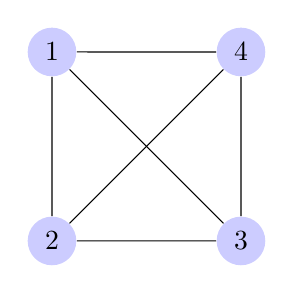
\begin{tikzpicture}
[scale=.8,every node/.style={circle,fill=blue!20}]
\node (n1) at (4,9) {1};
\node (n2) at (4,6) {2};
\node (n3) at (7,6) {3};
\node (n4) at (7,9) {4};
\foreach \from/\to in {n1/n2,n1/n3,n1/n4,n2/n3,n2/n4,n3/n4}
\draw (\from) -- (\to);
\end{tikzpicture}

we see that $\alpha(G) = 1$. But since this graph is complete, we see that if we delete any edge, we can get an independent set of size 2 by making the set include the two vertices that were connected by the edge we deleted. For example:

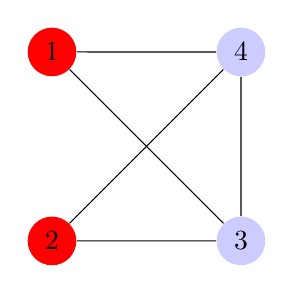
\begin{tikzpicture}
[scale=.8,every node/.style={circle,fill=blue!20}]
\node[fill = red] (n1) at (4,9) {1};
\node[fill = red] (n2) at (4,6) {2};
\node (n3) at (7,6) {3};
\node (n4) at (7,9) {4};
\foreach \from/\to in {n1/n3,n1/n4,n2/n3,n2/n4,n3/n4}
\draw (\from) -- (\to);
\end{tikzpicture}

Thus, G is $\alpha-$critical.
\end{exmp}

\begin{lemma}
\label{alpha}
If G is $\alpha-$critical, and $W$ an optimal weight matrix of G, then $w_{i,j} \neq$ 0 for all $i,j \in E(G)$
\end{lemma} 
\begin{proof}
Assume for the sake of contradiction, that for some $i,j \in E(G)$, we have $w_{i,j} = 0$. Then, we know $\alpha(G-e_{i,j}) > \alpha(G)$ because G is $\alpha-$critical. Thus:

$\alpha(G) < \alpha(G-e_{i,j}) \leq \min\{|G| - n_+(W),|G| - n_-(W)\}$

Thus, we see that the inertia bound is not tight for G, so W is not an optimal weight matrix of G, which is a contradiction.
\end{proof}

Due to the complexity of needing to consider edges that could potentially be zero in the weight matrix, it is easier to consider graphs that are restricted to only non-zero edge weights in its optimal weight matrix. Thus, it makes sense to only consider $\alpha-$critical graphs, because of Lemma \ref{alpha} ensuring that all $\alpha-$critical graphs have non-zero weight matrices.

\subsubsection{Determining Each Triangle Must Have the Same Sign}


\subsection{Graphs Currently Found}

\renewcommand{\thempfootnote}{\arabic{mpfootnote}}
\begin{center}
\begin{minipage}{\textwidth}
\small
\begin{tabular}{ |p{1cm}|p{1.5cm}|p{0.5cm}|p{1.5cm}|p{2.7cm}|p{2cm}|p{1cm}|} 
 \hline
 Graph & Vertices & $\alpha$ & Degree & Circulant & Strongly Regular & Arc Transitive\\ 
 \hline
 \footnote{Otr@PKoE?T\_iOoOG\_dg\_m\label{graph1}} & 16 & 4 & 5 & No & No & No\\
 \hline
 \footnote{O$\sim\sim$em]uj[vmsZTUrfFwN$\sim$\label{graph2}} & 16 & 2 & 10 & No & (16,10,6,6) & Yes \\
 \hline
 \footnote{P\}qtSeLUbaKeQZJabfGmmG$\sim$G\label{graph3}} & 17 &  3 & 8 & [1,2,4,8] & (17,8,3,4) & Yes\\
 \hline
 \footnote{R\}ecZ@OH?o\`W@gOWcI\_\`p?hkHL?GuG\label{graph4}} & 19 & 4 & 6 & [1,7,8] & No & Yes \\
 \hline
 \footnote{S$\sim\sim$vVjjve\}vmxymlG$\sim$Oi$\sim$Qm\{jfxjNw\{z\{\label{graph5}} & 20 & 2 & 13 & No & No & No\\
 \hline
 \footnote{S$\sim\sim$vnZjvUtvimj`$\sim$nibtTP\}[ffwk$\sim$wR$\sim$\{\label{graph6}} & 20 & 2 & 13 & [1,3,4,7,8,9,10] & No & No\\
 \hline
 \footnote{Uv$\sim$LnbgfeDShP\textbackslash{}G\}HuXmePrSemapSxqJWG$\vert$ZCVhw\label{graph7}} & 22 & 3 & 11 & [1,2,3,5,10,11] & No & No\\
 \hline
 \footnote{Wunneyzx$\sim$W]OwBPfcroK$\sim$S\{OlogtIoyPlPFMIIjWPUvaGu$\sim$\label{graph8}} & 24 & 3 & 12 & No & No & No\\
 \hline
 \footnote{WvrlvjZj$\sim$c\textbackslash{}\_wBTRcroK$\sim$K\{HLpGtPo[ikpImQHrWaUn`Cv\^{}\label{graph9}} & 24 & 3 & 12 & No & No & No\\
 \hline
 \footnote{WvvdtIJpB\_c[LEHPiH?PsE\_GAsWKcwBXhGDgOFXWIBV@CZT\label{graph10}} & 24 & 4 & 9 & No & No & No\\
 \hline
 \footnote{W\}mKmIbqD\_JJMMBYa]\_\{??ucC\{YKeHKXPadVXOmqQbqEDMp\label{graph11}} & 24 & 4 & 10 & [1,2,4,8,9] & No & No\\
 \hline
 \footnote{W\}nS$\vert$QeoOq\_nWS]?KcPQUPDgU@\_TBG\_ug@ei?jCgCwY\_?J$\sim$\label{graph12}} & 24 & 4 & 9 & No & No & No\\
 \hline
 \footnote{W\}\}VNbMtdyWkic?zg]gevHT\_TfGo$\sim$bPK$\vert$xHkJJMolozdq\textbackslash{}s\label{graph13}} & 24 & 3 & 12 & No & No & No\\
 \hline
 \footnote{W\}$\sim$SvAbp@IcjDgEaj?@BKPCgBbXP@oCz?BLdE@KwGu[?EFZ\label{graph14}} & 24 & 4 & 9 & No & No & No\\
 \hline
 \footnote{W$\sim$nELU\textbackslash{}`aKkXTJ]?@cGUB@KgBSX?wG\_sS`DUCGyWO`\}?@M\^{}\label{graph15}} & 24 & 4 & 9 & No & No & No\\
 \hline
 \footnote{W$\sim\sim\sim$vnnv$\vert$$\sim$\}gzH\}`za$\vert$J\^{}ef$\vert\sim$wBJNisn[bn\^{}@\^{}nwez$\sim$`V\^{}$\sim$\label{graph16}} & 24 & 2 & 16 & No & No & No\\
 \hline
 \footnote{W$\sim\sim\sim$vnn\{vT\{nvFnFo\^{}\}$\sim$Dnw\textbackslash{}\{\^{}AF$\vert$hFz[YZ$\sim$DT$\sim$wX\^{}$\sim$n\{B$\sim$\label{graph17}} & 24 & 2 & 16 & No & No & No\\
 \hline
 \footnote{W$\sim\sim\sim$vnn\{vXyjqnnFs\^{}\}$\sim$Knw\textbackslash{}[\^{}QF$\vert$hiz[iznCt$\sim$wX\^{}$\sim$n\{B$\sim$\label{graph18}} & 24 & 2 & 16 & [1,2,3,4,6,7,8,10] & No & No\\
 \hline
 \footnote{W$\sim\sim\sim$vvu$\vert$\^{}\textbackslash{}\textbackslash{}jvivTvtTyj\_$\sim\vert$\}ibyiiF\}[b\{$\sim$C\{$\sim$wU\^{}$\sim$\_f$\sim\sim$\label{graph19}} & 24 & 2 & 16 & No & No & No\\
 \hline
\end{tabular}
\end{minipage}
\end{center}

\subsubsection{Graphs Created from Deleting a Vertex}

\renewcommand{\thempfootnote}{\arabic{mpfootnote}}
\begin{center}
\begin{minipage}{\textwidth}
\begin{tabular}{ |p{1cm}|p{1.2cm}|p{1.5cm}|p{0.5cm}|p{1.5cm}|p{2.7cm}|p{2cm}|p{1cm}| } 
 \hline
 Graph & Created From & Vertices & $\alpha$ & Regular & Circulant & Strongly Regular & Arc Transitive\\ 
 \hline
 \footnote{Ntr@PKoE?T\_iOoOG\_dg\label{del1graph1}} & \ref{graph1} & 15 & 4 & No & No & No & No\\
 \hline
 \footnote{N$\sim\sim$em]uj[vmsZTUrfFw\label{del1graph2}} & \ref{graph2} & 15 & 2 & No & No & No & No\\
 \hline
 \footnote{O\}qtSeLUbaKeQZJabfGmm\label{del1graph3}} & \ref{graph3} & 16 & 3 & No & No & No & No\\
 \hline
 \footnote{Q\}ecZ@OH?o\`W@gOWcI\_\`p?hkHL?\label{del1graph4}} & \ref{graph4} & 18 & 4 & No & No & No & No\\
 \hline
 \footnote{R$\sim\sim$vnZjvUtvimj`$\sim$nibtTP\}[ffwk$\sim$w\label{del1graph5}} & \ref{graph6} & 19 & 2 & No & No & No & No\\
 \hline
 \footnote{Tv$\sim$LnbgfeDShP\textbackslash{}G\}HuXmePrSemapSxqJWG$\vert$Z\label{del1graph6}} & \ref{graph7} & 21 & 3 & No & No & No & No\\
 \hline
 \footnote{Vunneyzx$\sim$W]OwBPfcroK$\sim$S\{OlogtIoyPlPFMIIjWPUv\_\label{del1graph7}} & \ref{graph8} & 23 & 3 & No & No & No & No\\
 \hline
  \footnote{VvrlvjZj$\sim$c\textbackslash{}\_wBTRcroK$\sim$K\{HLpGtPo[ikpImQHrWaUn\_\label{del1graph8}} & \ref{graph9} & 23 & 3 & No & No & No & No\\
 \hline
  \footnote{VvvdtIJpB\_c[LEHPiH?PsE\_GAsWKcwBXhGDgOFXWIBV?\label{del1graph9}} & \ref{graph10} & 23 & 4 & No & No & No & No\\
 \hline
  \footnote{V\}mKmIbqD\_JJMMBYa]\_\{??ucC\{YKeHKXPadVXOmqQbq?\label{del1graph10}} & \ref{graph11} & 23 &  4 & No & No & No & No\\
 \hline
  \footnote{V\}nS$\vert$QeoOq\_nWS]?KcPQUPDgU@\_TBG\_ug@ei?jCgCwY\_\label{del1graph11}} & \ref{graph12} & 23 & 4 & No & No & No & No\\
 \hline
  \footnote{W\}\}VNbMtdyWkic?zg]gevHT\_TfGo$\sim$bPK$\vert$xHkJJMolozdq\textbackslash{}s\label{del1graph12}} & \ref{graph13} & 23 & 3 & No & No & No & No\\
 \hline
  \footnote{V\}$\sim$SvAbp@IcjDgEaj?@BKPCgBbXP@oCz?BLdE@KwGu[?\label{del1graph13}} & \ref{graph14} & 23 & 4 & No & No & No & No\\
 \hline
  \footnote{V$\sim$nELU\textbackslash{}`aKkXTJ]?@cGUB@KgBSX?wG\_sS`DUCGyWO`\}?\label{del1graph14}} & \ref{graph15} & 23 & 4 & No & No & No & No\\
 \hline
  \footnote{V$\sim\sim\sim$vnnv$\vert$$\sim$\}gzH\}`za$\vert$J\^{}ef$\vert\sim$wBJNisn[bn\^{}@\^{}nwez$\sim$\_\label{del1graph15}} & \ref{graph16} & 23 & 2 & No & No & No & No\\
 \hline
  \footnote{V$\sim\sim\sim$vnn\{vT\{nvFnFo\^{}\}$\sim$Dnw\textbackslash{}\{\^{}AF$\vert$hFz[YZ$\sim$DT$\sim$wX\^{}$\sim$\_\label{del1graph16}} & \ref{graph17} & 23 & 2 & No & No & No & No\\
 \hline
  \footnote{V$\sim\sim\sim$vnn\{vXyjqnnFs\^{}\}$\sim$Knw\textbackslash{}[\^{}QF$\vert$hiz[iznCt$\sim$wX\^{}$\sim$\_\label{del1graph17}} & \ref{graph18} & 23 & 2 & No & No & No & No\\
 \hline
  \footnote{V$\sim\sim\sim$vvu$\vert$\^{}\textbackslash{}\textbackslash{}jvivTvtTyj\_$\sim\vert$\}ibyiiF\}[b\{$\sim$C\{$\sim$wU\^{}$\sim$\_\label{del1graph18}} & \ref{graph19} & 23 & 2 & No & No & No & No\\
 \hline
 \footnote{P\}ecZ@OH?o\`W@gOWcI\_\`p?hk\label{del2graph1}} & \textsuperscript{\ref{del1graph4}} & 17 & 4 & No & No & No & No\\
 \hline
 \footnote{Q$\sim\sim$vnZjvUtvimj`$\sim$nibtTP\}[ffw\label{del2graph2}} & \textsuperscript{\ref{del1graph5}} & 18 & 2 & No & No & No & No\\
 \hline
 \footnote{UvvdtIJpB\_c[LEHPiH?PsE\_GAsWKcwBXhGDgOFXW\label{del2graph3}} & \textsuperscript{\ref{del1graph9}} & 22 & 4 & No & No & No & No\\
 \hline
 \footnote{U\}nS$\vert$QeoOq\_nWS]?KcPQUPDgU@\_TBG\_ug@ei?jCg\label{del2graph4}} & \textsuperscript{\ref{del1graph11}} & 22 & 4 & No & No & No & No\\
 \hline
 \footnote{U$\sim\sim\sim$vnnv$\vert$$\sim$\}gzH\}`za$\vert$J\^{}ef$\vert\sim$wBJNisn[bn\^{}@\^{}nw\_\label{del2graph5}} & \textsuperscript{\ref{del1graph15}} & 22 & 2 & No & No & No & No\\
 \hline
 \footnote{U$\sim\sim\sim$vvu$\vert$\^{}\textbackslash{}\textbackslash{}jvivTvtTyj\_$\sim\vert$\}ibyiiF\}[b\{$\sim$C\{$\sim$w\label{del2graph6}} & \textsuperscript{\ref{del1graph18}} & 22 & 2 & No & No & No & No\\
 \hline
 \footnote{O\}ecZ@OH?o\`W@gOWcI\_\`p\label{del3graph1}} & \textsuperscript{\ref{del2graph1}} & 16 & 4 & No & No & No & No\\
 \hline
 \footnote{TvvdtIJpB\_c[LEHPiH?PsE\_GAsWKcwBXhGDg\label{del3graph2}} & \textsuperscript{\ref{del2graph3}} & 21 & 4 & No & No & No & No\\
 \hline
 \footnote{T$\sim\sim\sim$vvu$\vert$\^{}\textbackslash{}\textbackslash{}jvivTvtTyj\_$\sim\vert$\}ibyiiF\}[b\{$\sim$\label{del3graph3}} & \textsuperscript{\ref{del2graph6}} & 21 & 2 & No & No & No & No\\
 \hline
 
 
\end{tabular}
\end{minipage}
\end{center}

\section{Other Useful Information}

\subsection{Cayley Graphs}
\begin{definition}[Cayley Graph]
Let $H$ be a finite group, and $S \subseteq H$, be a subset of $H$. Then the Cayley Graph $C(H,S)$, has a vertex for each element in $H$. There exists an edge between two vertices $g$ and $h$, if and only if there exists $s \in S$ such that $ sh = g$. If $G$ is a graph such that there exists a group $H$ and a generating set $S \subseteq H$ with $G \cong C(H,S)$, then G is a Cayley Graph. \cite{franccayley}

\end{definition}

\begin{exmp}
Consider the group $\mathbb{Z}_8$ and let the generating set be $S = \{1,2\}$. The vertex set will be $\{0,1,2,3,4,5,6,7\}$ and there will be an edge between two vertices, $g$ and $h$, if for an $s \in S$, $g + s = h$:
\\

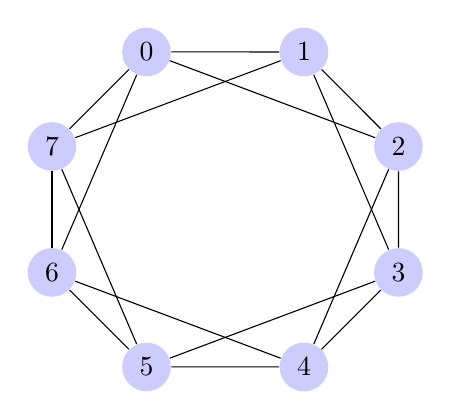
\begin{tikzpicture}
[scale=.8,every node/.style={circle,fill=blue!20}]
\node (n0) at (1.5,9) {0};
\node (n1) at (4,9) {1};
\node (n2) at (5.5,7.5) {2};
\node (n3) at (5.5,5.5) {3};
\node (n4) at (4,4) {4};
\node (n5) at (1.5,4) {5};
\node (n6) at (0,5.5) {6};
\node (n7) at (0,7.5) {7};
\foreach \from/\to in {n0/n1,n1/n2,n2/n3,n3/n4,n4/n5,n5/n6,n6/n7, n7/n0, n0/n2, n1/n3,n2/n4,n3/n5,n4/n6,n5/n7,n6/n0,n7/n1}
\draw (\from) -- (\to);
\end{tikzpicture}

\end{exmp}

\subsection{John's Proof}

\begin{definition}[k-saturated]
The graph $G$ is said to be $k$-saturated if it does not contain a complete $(k+1)$-graph, but every graph $G'$ obtained from adding a new edge to G contains a complete $(k+1)$-graph. \cite{kSaturated}
\end{definition}

\begin{definition}[Conical Vertex]
A vertex, $V$, is a conical vertex of a graph, $G$, if $V$ is adjacent to every vertex in $G$.
\end{definition}


\begin{observation} \label{obs-sat}
A graph, $G$, is $k$-saturated, if and only if its complement, $\overline{G}$, is $\alpha$-critical, with $\alpha(\overline{G})=k$. \\
This is due to the fact that since $G$ contains a complete $k$-graph but not a complete $(k+1)$-graph, $\overline{G}$ will have a maximum independent set of size $k$. By adding any edge to $G$ to obtain $G'$, $G'$ will contain a complete (k+1)-graph, and thus $\overline{G'}$ will then have an independent set of size $k+1$. Thus, $\overline{G}$ is $\alpha$-critical and $\alpha(G)=k$.
\end{observation}

\begin{theorem} \label{k-sat}
Assume $G$ is $k$-saturated. Then $G$ contains at least $2k - |G|$ conical vertices. \cite{kSaturated}
\end{theorem}

\begin{observation} \label{Contra}
From theorem \ref{k-sat}, thinking in terms of of the complement of a graph, we get that if $G$ is $\alpha$-critical and connected, then $G$ must satisfy $\alpha(G) \leq \frac{|G|}{2}$.
\end{observation}

\begin{proof}
Beginning with a graph $G$, if $G$ is $\alpha$-critical with $\alpha(G)=k$, then due to observation \ref{obs-sat}, $\overline{G}$ is $k$-saturated. Now, following from theorem \ref{k-sat}, $\overline{G}$ contains at least $2k - |\overline{G}|$ conical vertices. This means that $G$ must contain at least $2k - |\overline{G}| = 2\alpha(G) - |G|$ isolated vertices. However, $G$ is connected, so the number of isolated vertices must equal zero and so $2\alpha(G) - |G| \leq 0$. Rearranging, gives $\alpha(G) \leq \frac{|G|}{2}$ as required.
\end{proof}

As well, consider the contrapositive of the statement:
if $\alpha(G) > \frac{|G|}{2}$, then G is either not connected or not $\alpha$-critical.

\begin{theorem} \label{John's}
Let $G$ be a connected graph such that $\alpha(G) \geq \frac{|G|}{2}$. Then either $G$ has a tight weight matrix, or there exists an induced subgraph, $H$, such that $H$ has no tight weight matrix and $\alpha(H) < \frac{|H|}{2}$.
\end{theorem}

\begin{proof}

First off, following from \cite{plummer1970some}, the only graph, $H$, with $\alpha(H) = \frac{|H|}{2}$ is the complete graph, $K_2$. However, since $K_2$ has less than 10 vertices, we know that from \cite{elzinga2007minimum} that $K_2$ does not have a tight weight matrix. Thus, the statement is true for $K_2$ and since it is the only graph with $\alpha(K_2) = \frac{|K_2|}{2}$, we now only need to consider graphs, $G$, with $\alpha(G) > \frac{|G|}{2}$.

We will proceed with induction on the number of vertices.

Base case: Let $G$ be a connected graph on 10 vertices or less with $\alpha(G) > \frac{|G|}{2}$. Then from \cite{elzinga2007minimum}, we know that all graphs on 10 vertices or less does not have a tight weight matrix, and so G does not have a tight weighting.

Inductive Hypothesis: Let $G$ be a connected graph on n vertices such that $\alpha(G) > \frac{|G|}{2}$. Then either $G$ has a tight weight matrix, or there exists an induced subgraph, $H$, such that $H$ has no tight weight matrix and $\alpha(H) \leq \frac{|H|}{2}$.

Inductive Step: Consider a connected graph $G$ on n+1 vertices such that $\alpha(G) > \frac{|G|}{2}$. Now if G has a tight weight matrix, we're done, so assume that G does not have a tight weight matrix. Now, from the contrapositive of observation \ref{Contra} and due to $G$ being connected, we know $G$ is not $\alpha$-critical. Thus, there exists an edge, $e_1$, such that $\alpha(G-e_1) = \alpha(G)$. This leaves us with 2 cases:

Case 1: $G-e_1$ is disconnected. In this case, either both of the components have a tight weighting, or at least one has a non-tight weighting. If one has a non-tight weight matrix, then $G$ contains an induced subgraph, $H$, such that $H$ has no tight weight matrix. Now, either $H$ satisfies $\alpha(H) \leq \frac{|H|}{2}$ in which case we're done, or $\alpha(H) > \frac{|H|}{2}$. If $\alpha(H) > \frac{|H|}{2}$, then we apply the inductive hypothesis to $H$ and since we already know $H$ does not have a tight weight matrix, it must be the case the $H$ contains an induced subgraph $F$ such that $F$ has no tight weight matrix and $\alpha(F) \leq \frac{|F|}{2}$. However, since $F$ is an induced subgraph of $H$, it must also be an induced subgraph of $G$, and so we find that $F$ satisfies the condition that $G$ has an induced subgraph with $\alpha(F) \leq \frac{|F|}{2}$ and so we are done. Thus, assume that both components have a tight weighting. However, using both of these tight weightings on $G$, and setting $e_1$ to a zero weighting, $G$ then has a tight weight matrix. However, this is a contradiction as we assumed $G$ did not have a tight weight matrix. This completes this case.

Case 2: $G-e_1$ is connected. Now because $G$ was not $\alpha$-critical, $\alpha(G) = \alpha(G-e_1)$ and so $\alpha(G-e_1) > \frac{|G-e_1|}{2}$. Thus, due to observation \ref{obs-sat}, $G-e_1$ is still not $\alpha$-critical. Therefore, we can continue to delete edges without changing the fact that the resulting graph will be $\alpha$-critical as long as it's connected. Now, consider the graph that results from $G$, which will be denoted $G'$, where after deleting $k-1$ edges, $G$ is still connected, but after deleting the $kth$ edge, $G$ has now become disconnected. We can now add back all edges that do not reconnect $G'$ as this will not decrease $\alpha(G')$ since deleting it did not. Now, we have the same situation as Case 1, with the only difference being that if the two disconnected components of $G'$ have a tight weighting, we use their tight weightings and put the weightings of all edges we deleted to obtain $G'$ to 0, giving us a tight weighting for $G$. This completes this case. \\

Therefore, $G$ satisfies the statement, and so by induction, the statement is true for all graphs.
\end{proof}

\subsection{No Bound on Inertia Bound Gap}

\begin{theorem}
For a graph $G$, there does not exist a bound on the difference between $\alpha(G)$ and the minimum inertia of a weight matrix corresponding to $G$.
\end{theorem}

\begin{proof}
Consider a graph, $G$, such that $G$ does not have a tight weight matrix with the gap from equality in the inertia bound being $\gamma$, and G-v does not have a tight weight matrix and $\alpha(G) = \alpha(G-v)$ $\forall v \in V(G)$. Paley 17 is an example of a graph that has this property so there will exist such a graph. Now, construct a graph $H$ by connecting two copies of $G$, $G_1$ and $G_2$, with an edge between a vertex on each copy of $G$ that does not belong to the independent set of either $G_1$ or $G_2$.

Now, consider the induced subgraph $H'$ obtained by deleting the vertex from the component $G_1$ in $H$ that connects to the cut-edge in $H$. This will result in $H'$ having two components, $G_1-v$ and $G_2$. Now any weight matrix of $H'$, $W'$ will have the form:

\begin{center}
$W'=
\begin{bmatrix}
W_1 & 0 \\
0 & W_2 \\
\end{bmatrix}
$
\end{center}

With $W_1$ and $W_2$ being the weight matrices associated with the components $G_1-v$ and $G_2$, respectively. As a result, the eigenvalues of $W'$ will be equal to the eigenvalues of $W_1$ and $W_2$. Thus, for any weight matrix $W'$ of $H'$, the inertia of $W'$ will be equal to the sum of the inertias of $W_1$ and $W_2$. Therefore,
\begin{multline}
\min\{|H'|-n_+(W'), |H'|-n_-(W')\} \\ = \min\{|G-v|-n_+(W_1), |G-v|-n_-(W_1)\} + \min\{|G|-n_+(W_2), |G|-n_-(W_2)\} \\ \leq 2\min\{|G|-n_+(W_2), |G|-n_-(W_2)\}
\end{multline}
From Cauchy's Eigenvalue Interlacing Theorem , we know any weight matrix associated with $H$, $W$, will have at least as many positive and negative eigenvalues as $W'$. Thus,
\begin{multline}
\min\{|H'|-n_+(W'), |H'|-n_-(W')\} \\ \leq 2\min\{|G|-n_+(W_2), |G|-n_-(W_2)\} \\ \leq \min\{|H|-n_+(W), |H|-n_-(W)\}
\end{multline}
Due to how we created $H$, $\alpha(H) = 2\alpha(G)$ because the largest independent set of $H$ will just equal the union of the largest independent set of $G_1$ and $G_2$ since we connected $G_1$ and $G_2$ without connecting edges between the two independent sets.

Therefore, we get:

\begin{center}
\begin{multline}
\alpha(H) \\ = 2\alpha(G) \\ = 2\gamma + 2\min{|G|-n_+(W_2), |G|-n_-(W_2)} \\ \leq 2\gamma + \min\{|H|-n_+(W), |H|-n_-(W)\}
\end{multline}
\end{center}

Therefore, the gap between equality in the inertia bound has at least doubled. Now as long as there exists a graph without a tight weight matrix, $F$, such that $F-v_1-v_2$ also does not have a tight weight matrix, we can generalize this result to create a new graph, connecting arbitrarily many copies of $F$ and following the same argument to multiply the gap in the inertia bound by how many copies of $F$ we connect.

\end{proof}

\bibliographystyle{plain}
\bibliography{mybib}

\end{document}



